\chapter[Experimental methods]{Experimental methods}
\markboth{Chap. 3\ \ \enspace Experimental methods}{Chap 2. Experimental methods}

\regularsection
\headerregularsection

\updatemylof % to be used with "list of figure divider per chapter" (see PREAMBLE)
\updatemylot % to be used with "list of table divider per chapter" (see PREAMBLE)

\begin{sloppypar} % to suppress overfull box

Lorem \index{Lorem} ipsum dolor sit amet, consectetuer adipiscing elit \cite{LIUDIMULYO201767}. Ut purus \index{purus} elit,vestibulum ut, placerat ac, adipiscing vitae, felis \citenum{LIUDIMULYO201767}. Curabitur dictum \index{dictum} gravidamauris. Nam arcu libero, nonummy eget, consectetuer id, vulputate a, magna. Donec vehicula augue eu neque \cite{liudimulyo_2018}. Pellentesque habitant morbi tristique senectuset netus et malesuada fames ac turpis egestas \index{egestas}\citenum{liudimulyo_2018}. Mauris ut leo. Cras viverra metusrhoncus sem \cite{2019liudimulyo}. Nulla et lectus vestibulum urna fringilla ultrices. Phasellus eutellus sit amet tortor gravida placerat \citenum{2019liudimulyo}. Integer sapien est, iaculis in, pretium quis,viverra ac, nunc. Praesent eget sem vel leo ultrices bibendum \cite{liudimulyo2020853}. Aenean faucibus. Morbi dolor nulla, malesuada eu, pulvinar at (\ref{fig:figures/paper-iv/fig-3}), mollis ac, nulla. Curabitur auctorsemper nulla \citenum{liudimulyo2020853}. Donec varius orci eget risus. Duis nibh mi, congue eu, accumsaneleifend, sagittis quis, diam. Duis eget orci sit amet orci dignissim rutrum \cite{LIUDIMULYO201767,liudimulyo_2018,2019liudimulyo,liudimulyo2020853,liudimulyo_unpublished1,liudimulyo_unpublished2}.

\end{sloppypar}

\begin{figure}[H] % \begin{figure}[H] for forcing the figure placement here ; in the bottom, \begin{figure}[!b] ; top of the page, \begin{figure}[!t] ; otherwise, \begin{figure} will let LaTeX decide the best figure placement for you
    \centering
    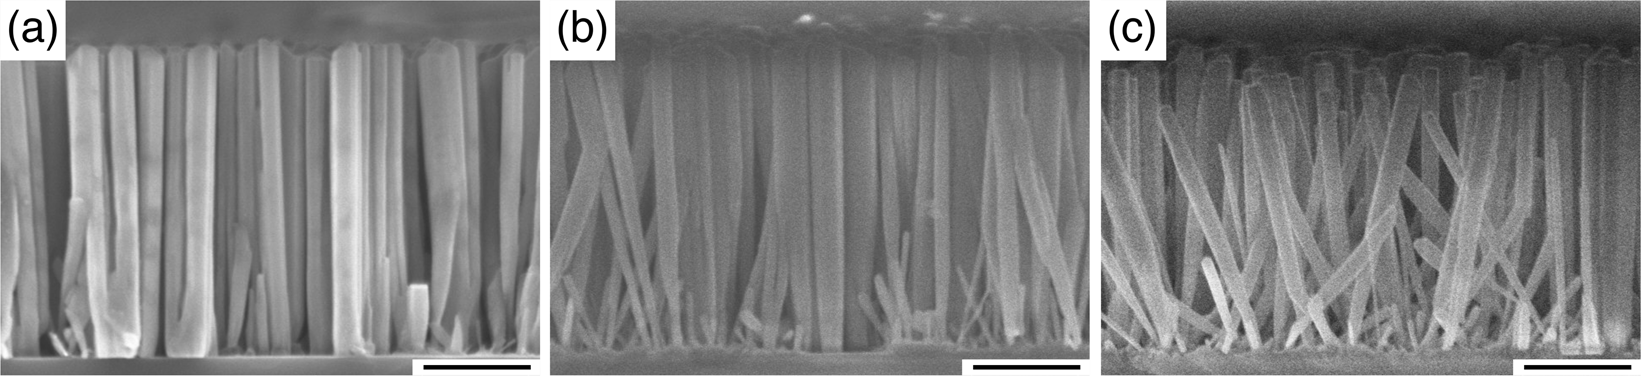
\includegraphics[width=\textwidth]{figures/paper-iv/fig-3.png}
    \caption[Cross-sectional SEM images of GaN nanocolumns on graphene formed via different AlN MEE cycles]{Cross-sectional SEM images of GaN nanocolumns on graphene formed via different AlN MEE cycles. Samples (\textbf{a}) G1, (\textbf{b}) G2, and (\textbf{c}) G3. Scale bars are 500 nm (adapted with permission from ref. \citenum{liudimulyo2020853} \copyright \ Liudi Mulyo \textit{et al}, 2020.}
    \label{fig:figures/paper-iv/fig-3}
\end{figure}

\section{Section 1 in chapter 3}
\lipsum[2]

\begin{equation}
    EQE = \frac{q \times P_{opt}}{I \times h\nu}
\end{equation}

\lipsum[3]
\ref{tab:ch3} lists the experimental conditions of each sample synthesized in this study.

\begin{table}[!h]
\centering
\caption[Experimental conditions described in the ToC]{Experimental conditions.}
\label{tab:ch3}
{\renewcommand{\arraystretch}{1.3}
\begin{tabular}{@{}*{8}{p{.125\textwidth}@{}}}
\toprule
\textbf{Sample ID} & A1    & A2    & A3    & A4    & A5    & A6    & A7    \\
\textbf{T\textsubscript{sub} ($^\circ$C)}  & 100      & 110      & 120      & 130      & 140      & 150      & 160      \\
\textbf{\textPhi\textsubscript{Ga} (Pa)}   & 1.0$\times$10\textsuperscript{-10} & 1.0$\times$10\textsuperscript{-11} & 1.0$\times$10\textsuperscript{-12} & 1.0$\times$10\textsuperscript{-13} & 1.0$\times$10\textsuperscript{-14} & 1.0$\times$10\textsuperscript{-15} & 1.0$\times$10\textsuperscript{-15} \\
\textbf{Q\textsubscript{N} (sccm)} & 1.5     & 1.6     & 1.7     & 1.8     & 1.9     & 2.00     & 2.1 \\
\bottomrule
\end{tabular}
}
\end{table}

\subsection{Subsection 3.1 of section 1 in chapter 3}
\lipsum[5-7]

\subsection{Subsection 3.2 of section 1 in chapter 3}
\lipsum[8-9]

\clearpage\phantomsection % to fix wrong hyperref to this section
\section[Long section title displayed in the table of content]{Short section title in the chapter}
\sectionmark{Even shorter title on the header}
\lipsum[11-20]

\subsection{Subsection 3.2 of section 2 in chapter 3}
\lipsum[13-14]

%=======================================================================
%%% References 

% \clearpage
\phantomsection
\specialsection % put an indent, see preamble
\headerspecialsection

{\hypersetup{urlcolor=ntnu,linkcolor=sophia} % set clickable URL title color to black, not ntnu like in the main document

\bibliographystyle{unsrtnat-mod}  % NATBIB ref style
\bibliography{references}
}